\chapter{Dynamic Maps User Study}
\label{chap:userStudy}

\bibentry{mcnabb2018when} \cite{mcnabb2018when}  \\

\chapterquote{If you can't read the scoreboard. You don't know the score. If you don't know the score, you can't tell the winners from the losers.}
{Warren Buffet, CEO of Berkshire Hathaway}

\newpage
{\footnotesize \hypersetup{linkcolor=black}
\minitoc}

%\begin{abstract}
%\newpage
%\topskip0pt
%\vspace*{4cm}
%\section*{Chapter Abstract}
%Choropleth maps are an invaluable visualization type for mapping geo-spatial data. One advantage to a choropleth map over other geospatial visualizations such as cartograms is the familiarity of a non-distorted landmass. However, this causes challenges when an area becomes too small in order to accurately perceive the underlying color. When does size matter in a choropleth map? We conduct an experiment to verify the relationship between choropleth maps, their underlying color map, and a user's perceivability. We do this by testing a user's perception of color relative to an administrative area's size within a choropleth map, as well as user-preference of fixed-locale maps with enforced minimum areas. Based on this initial experiment we can make the first recommendations with respect to a unit area's minimum size in order to be perceivably useful.
%%\end{abstract}

\newpage

\section{Introduction} \label{sec:introduction}
 \begin{figure*}[ht]
  \centering
  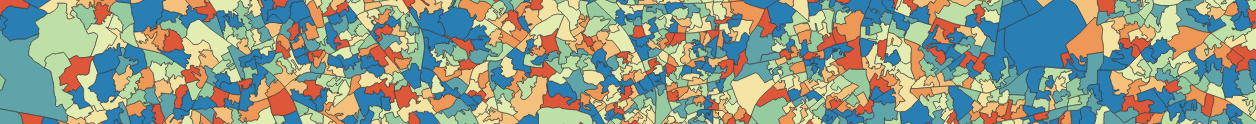
\includegraphics[width=\linewidth]{images/CypressView2}
  \caption{Presents a subset of administrative areas in London at 1.5\% of the scale of the full map.}
	\label{fig:teaser}
\end{figure*}

Having a completed algorithm for unifying areas based on scale, we verify its effectiveness for choropleth maps. First, we design a user study to present why it is helpful. We can do this by testing user task performance accuracy for small scale areas on a choropleth map. Secondly, we can review user preference of scale exploiting the algorithm in Chapter \ref{chap:dcm}.

Size is an important facet of visual design in visualization. Our survey of surveys finds scalability as the 3$^{rd}$ most cited future work direction across 40 visualization survey papers, only being preceded by evaluation and missing scenarios in classifications (Chapter \ref{chap:SoS}). In relation to choropleth maps, size is considered a widely recognized challenge in the field. Ward et al. state ``\textit{A problem of choropleth maps is that the most interesting values are often concentrated in densely populated areas with small and barely visible polygons}" \cite{ward2010interactive}. Lee \textit{et al.} suggest that improving tiny classes would be interesting future work in the field \cite{lee2013perceptually}.

We conduct a preliminary user-experiment to determine the minimum screen size of a unit area on a choropleth map in order to be accurately perceivable. We also measure the range of unit area sizes where an increase in perceivability error occurs. The experiment focuses on the scalability factors `human perception' and `monitor resolution', presented by Eick and Karr \cite{eick2002visual}.  We base our user-study on the following hypotheses:
\begin{itemize}[labelindent=1em, labelsep=0.2cm, leftmargin=*]
\item[\textbf{H1}]The smaller the size of a unit area, the higher the error rate of perceiving the correct underlying color category.
\item[\textbf{H2}]The smaller unit area, the more time required to perceive its color.
\item[\textbf{H3}]The user will prefer choropleth maps with a larger minimum size over those with smaller sizes. Particularly, users will prefer a trade-off between area resolution in favor of legibility.
\end{itemize}

The contributions of this chapter include:
\begin{itemize}[labelindent=1em, labelsep=0.2cm, leftmargin=*]
\item[\textbf{1.}] The first user-study of its kind to evaluate perceivability of color on a choropleth map relative to unit area size.
\item[\textbf{2.}] The first recommendation on the minimum screen space size a unit area should occupy to maintain perceivability on a choropleth map.
\item[\textbf{3.}] The first recommendation on the minimum screen space size a unit area should be to optimize user satisfaction.
\end{itemize}

The rest of the chapter is organized as follows. In Section \ref{sec:related}, we explore work in the related fields of perception of choropleths, color, and size. Section \ref{sec:tasks} breaks down the tasks that we will cover in our user study. Section \ref{sec:variables} describes the important variables that are considered in the user study, this is divided into dependent variables and controlled variables. In Section \ref{sec:experiment}, we discuss the procedure of our user study. We provide depth for each task in order to allow the study to be reproduced. In Section \ref{sec:stored}, we discuss the stored data from the experiments to give an understanding of the results. We then discuss the results of our three tasks in Section \ref{sec:results} in detail, and present our user-study findings. Finally, we give our conclusions. 

\section{Background} \label{sec:related}
We first describe previous research involving user-studies and perception. Chapter \ref{chap:SoS}, as well as Kijmongkolcahi \textit{et al.} \cite{kijmongkolchai2017empirically} provide papers that aid in the search for related work in the areas of human-centered evaluation of choropleths, color, and perception of size.

\textbf{Perception of Choropleths: }
Rittschof and Kulhavy present a user-study which includes a comparison of choropleth maps and cartograms. Cartograms are a different class of geo-visualization because they use distortion to convey data. They study the recall of data using different types of maps, firstly testing maps against the raw data and secondly studying two different map types (cartograms and choropleths) with two variations of exposure time.  Their results indicate that choropleth maps are associated with greater recall of information \cite{rittschof1998learning}. Kasper reviews the effectiveness of Gastner-Newman diffusion cartograms \cite{gastner2004diffusion} for the representation of population data which includes a comparative experiment against thematic maps (choropleth with overlayed circle maps) \cite{kaspar2011empirical}. The experiment is performed using two informatically equivalent maps using different designs, testing response times and accuracy for varied levels of question difficulty (using Bertin's map reading levels \cite{bertin1983semiology}). The results report that the thematic maps are more efficient and effective, particularly with complex tasks. Sun and Li review the effectiveness of cartograms for the representation of spatial data which includes a comparative experiment against thematic maps, including choropleths \cite{sun2010effectiveness}. The test takes place online for 100 subjects, who rank thematic maps (including choropleth maps) against cartograms. The results indicate that the thematic maps are more effective representing quantitative data whilst cartograms are more effective with qualitative data.

\textbf{Perception of Color: }
We find two survey papers related to color mapping and perception in visualization. Zhou and Hansen present a survey of color maps and color-map generation techniques in visualization, providing a helpful reference for readers who are faced with color mapping decisions \cite{zhou2015survey}. Silva \textit{et al.} presents an overview of color, color scales, and tools to guide expert and non-expert users \cite{silva2011using}. The paper examines different domains of visualization individually.

Heer and Stone investigate how a model of color-naming can enable user interfaces to meaningfully mimic a link between visual perception and symbolic cognition. Color saliency is used to define the degree to which a color value is uniquely named. This is tested against several popular qualitative and quantitative color palettes to find the average salience which is calculated using the algorithms provided in the paper \cite{heer2012color}. Lee \textit{et al.} present a color optimization algorithm for visibility measures over a range of color palettes \cite{lee2013perceptually}. They look at classes and the area the class will envelop, and modify the color palette based on this. Smaller classes are given higher saturation and luminance, for example. Fang \textit{et al.} provide an algorithmic approach for maximizing the perceptual distances among a set of colors, with a focus on color re-assignment, which may occur when values change, and the phenomenon of local maxima, which becomes a problem when new colors need to be added \cite{fang2017categorical}. Szafir presents quantitative studies measuring color difference perception for points, bars, and lines \cite{szafir2018modeling}. The experiment for each of the three marks is conducted using Amazon's Mechanical Turk with items of varying size in terms of pixels and recorded the distinguishability of the points, lines, and bars. The goal of the paper is the first step in discerning a quantitative understanding of color perception in visualization. Our paper is closely related to this, with a focus on the size of perceivable areas in color, and also focuses on maps rather than mark types.

\textbf{Perception of Size:}
Borgo \textit{et al.} present a new order of magnitude mark (OOMM) and an empirical study comparing logarithmic, linear, scale-stack, and their custom marks to test magnitude estimation, target identification, ratio estimation, and trend analysis \cite{borgo2014order}. The results found the  OOMM marks outperform state of the art techniques in quantitative analysis. Gramazio \textit{et al.} present a study looking at the relationship between perceivable size, grouping, and search performance. The user is asked to find a distinct mark amongst a set of distractor marks which was applied to a grid layout as well as a scattered layout \cite{gramazio2014relation}. The study finds that grouped, or single color layouts have a much faster response time, and visual marks below 0.508$^\circ$ showed a large drop in performance time. Jansen and Hornb{\ae}k provide a psychophysical investigation of size as a physical variable, where participants estimated size of objects between solid bars and spheres. Solid bars were found to be estimated based on their length whilst spheres were measured based on their surface area \cite{jansen2016psychophysical}.  Ronne Jakobsen and Hornb{\ae}k produce an experiment reviewing the use of overview+detail, focus+context, and zooming over 3 different display sizes. The results indicate that performance time for each technique was worse for smaller screens \cite{ronne2011sizing}. Healey and Sawant conduct an experiment to review identified pixel resolution and visual angle needed to distinguish different values of luminance, hue, size, and orientation \cite{healey2012on}. Our study differs by testing on a set of non-uniform shapes, as would be found on many choropleth maps.


\section{Experimental User Tasks} \label{sec:tasks}
We research the hypotheses presented in Section \ref{sec:introduction} by testing singular interpretation, comparative interpretation, and comparative preference using the following user tasks:
\begin{itemize}[labelindent=1em, labelsep=0.2cm, leftmargin=*]
\item[\textbf{T1}] Identify the color of a given unit area on a choropleth map.
\item[\textbf{T2}] Compare the relative color of two unit areas.
\item[\textbf{T3}] Select the preferred minimum size unit area on a dynamic choropleth map using a slider.
\end{itemize}
Details about how the tasks are performed can be found in Section \ref{sec:process}.

\begin{figure}[ht] \centering
\subfloat
{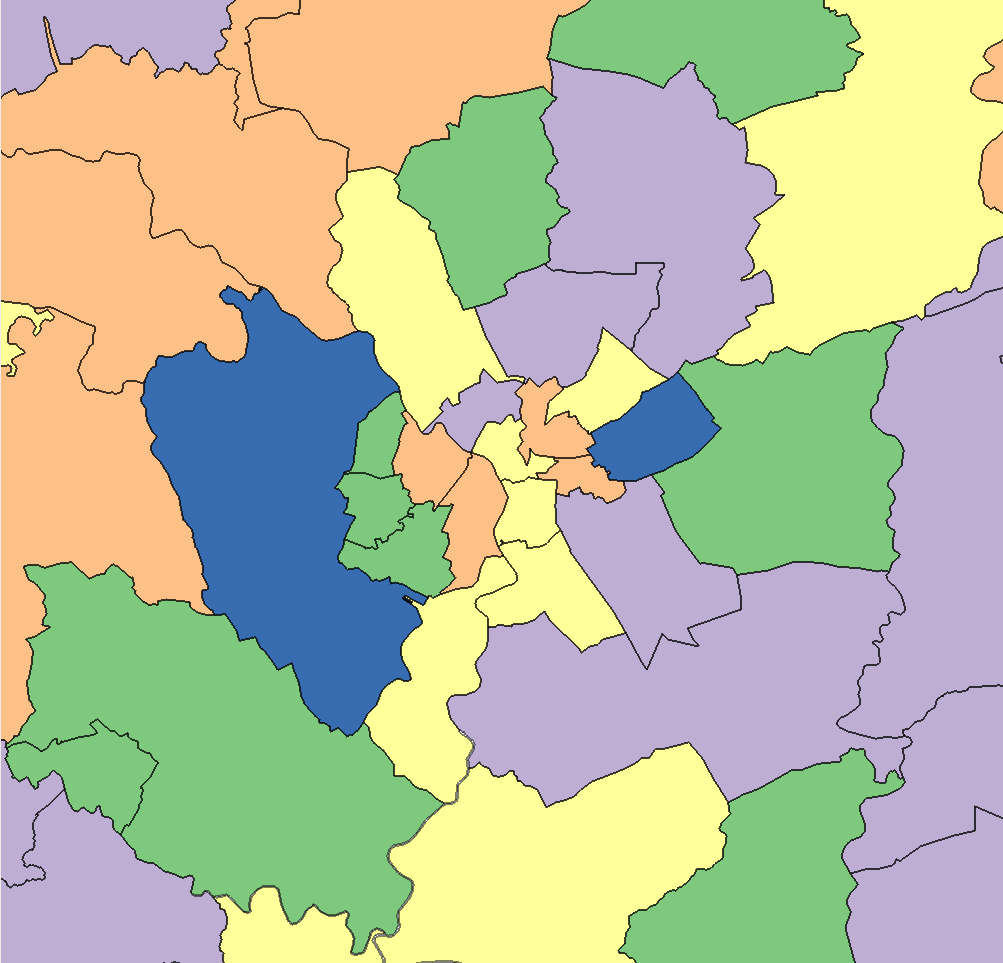
\includegraphics[width=0.3\linewidth]{images/boundaryBlack2}}
\subfloat
{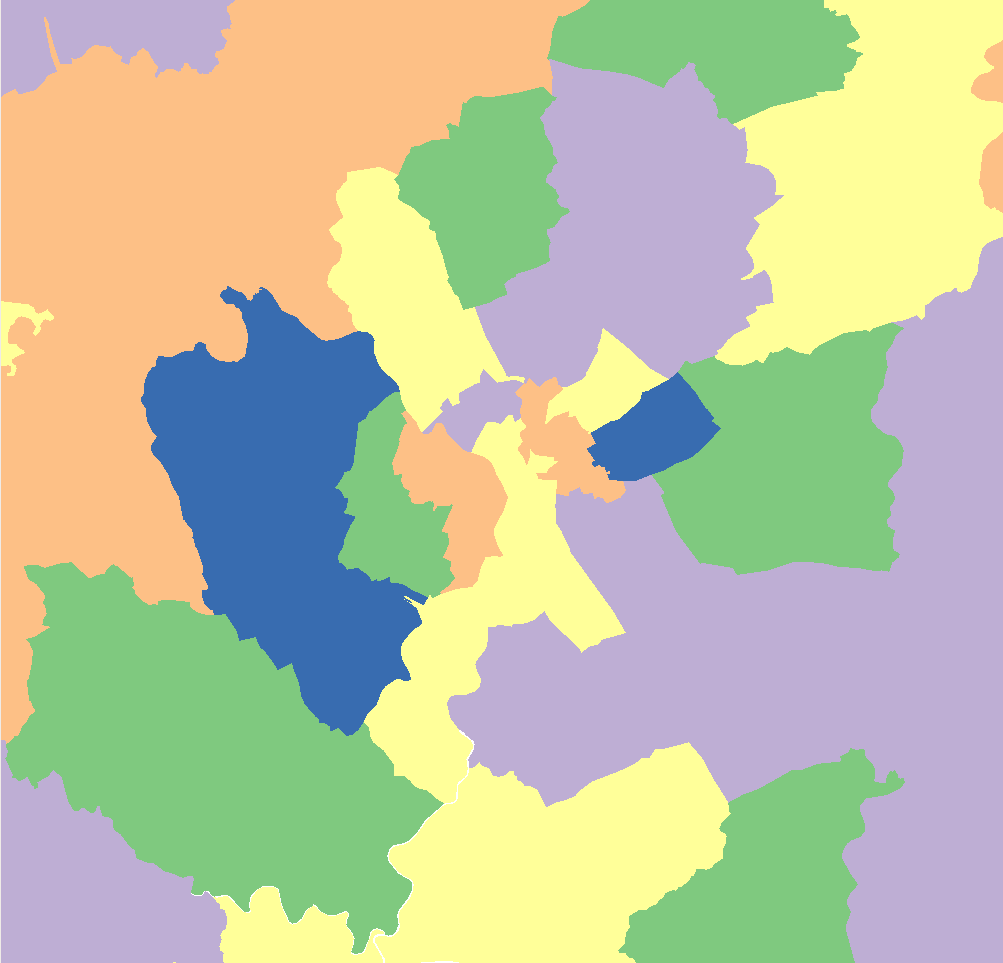
\includegraphics[width=0.3\linewidth]{images/boundaryNone2}}
\subfloat
{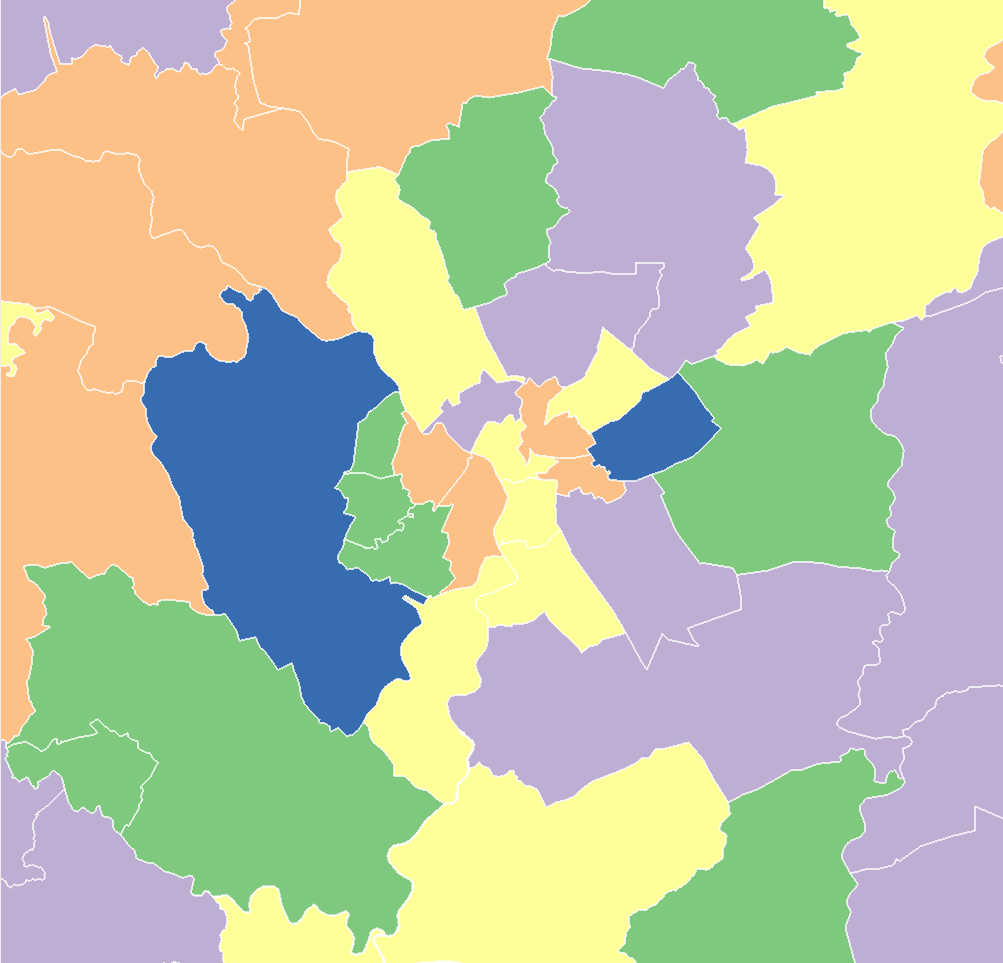
\includegraphics[width=0.3\linewidth]{images/boundaryWhite2}}\\ \setcounter{subfigure}{0}
\subfloat[Black Boundary]
{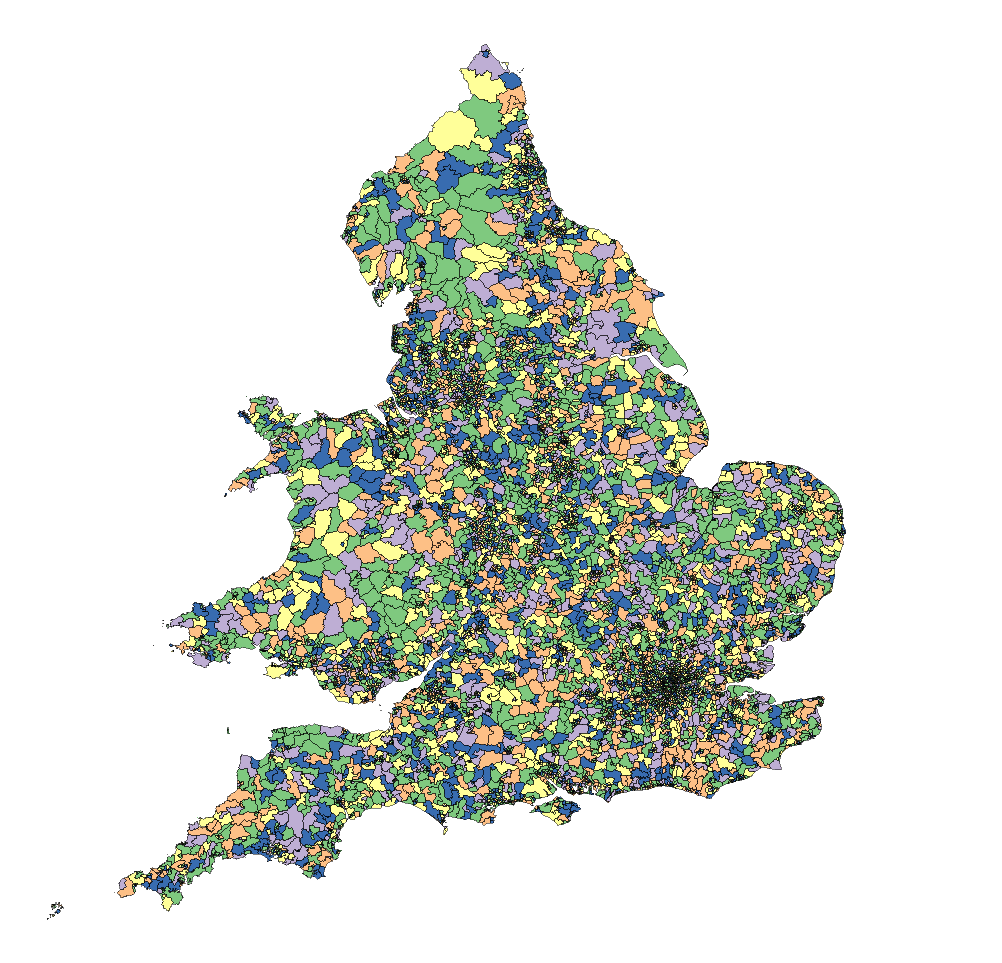
\includegraphics[width=0.3\linewidth]{images/FullBoundaryBlack}}
\subfloat[No Outline]
{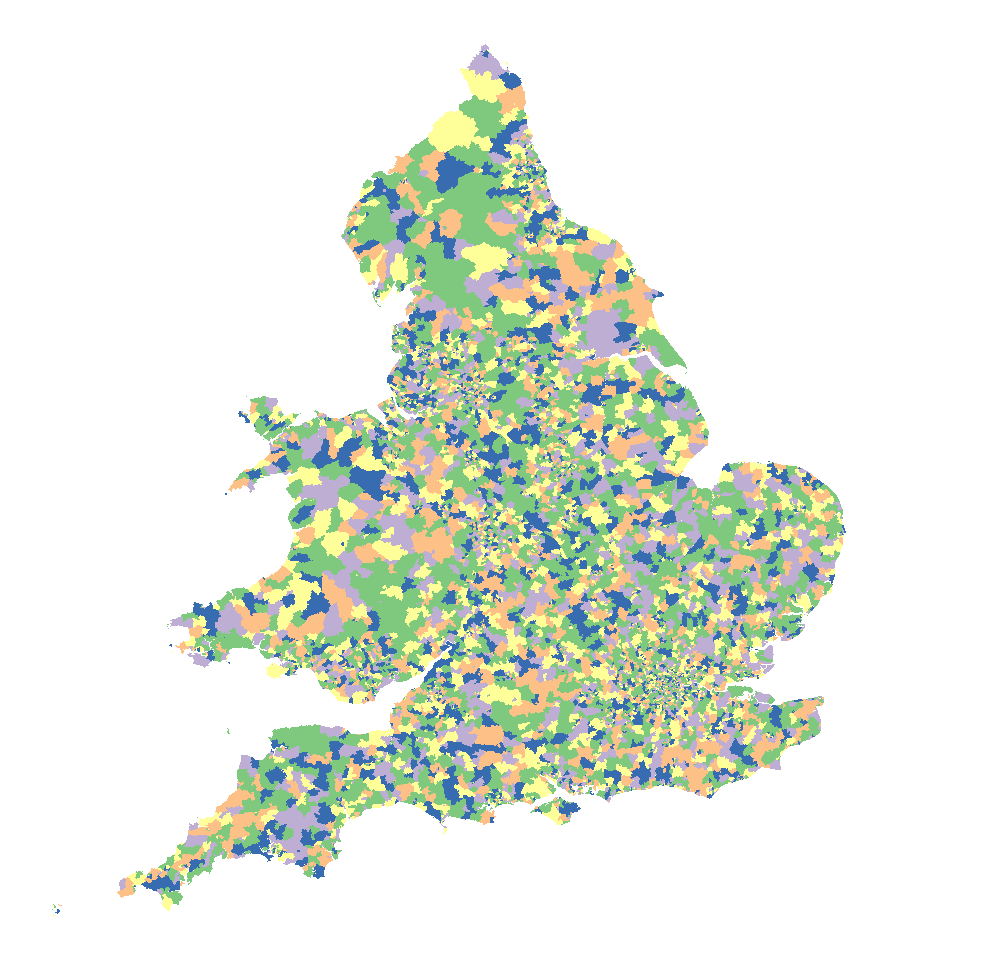
\includegraphics[width=0.3\linewidth]{images/FullBoundaryNone}}
\subfloat[Lower Alpha]
{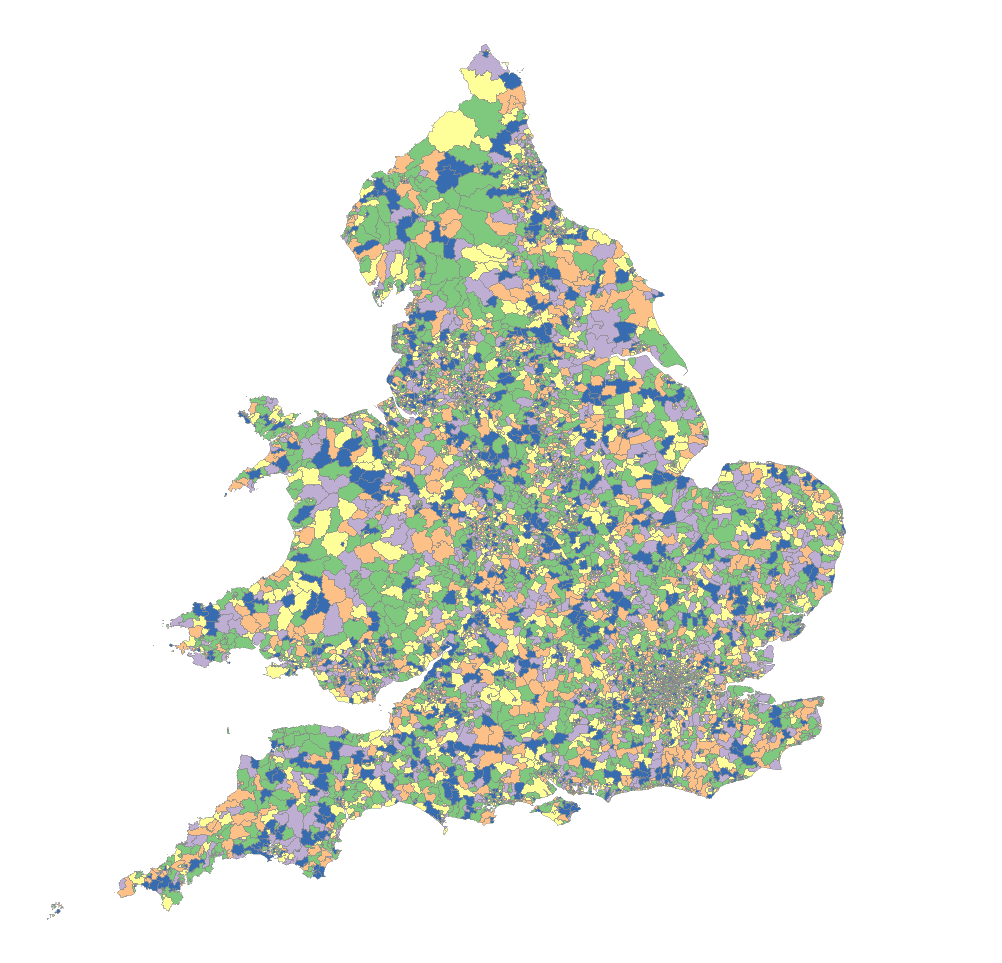
\includegraphics[width=0.3\linewidth]{images/FullBoundaryGrey}}
\caption{Three examples for boundary design at two different scales. The selected process is to use boundaries with a low alpha level. }\label{fig:boundaries}
\end{figure}

\begin{figure}[b]
\centering

\includegraphics[scale=1]{images/pixelSize} \vspace{0.1cm}
\caption{Area Size approximation demonstration.  (left) 1 pixel. (middle) 50 pixels. (right) 200 pixels} \label{fig:pixels}
\end{figure}
\section{Experimental Variables} \label{sec:variables}
In this section, we discuss the user-study variables, and some of the factors we consider in the design of the experiment. These are split into the dependent variables which we test, and variables we control.

\subsection{Dependent Variables}
Our primary dependent variable is the size of a unit-area on a choropleth map. The unit area size is an important attribute to study due to its common usage and variability in standard choropleth maps. We test variable unit-area sizes by looking at how small a unit area can be in order to perceive the color it encodes based on a given color-map. We measure the size in terms of the number of color-mapped pixels in a given unit area. This measure is somewhat screen dependent since different displays feature different pixel densities, thus we use the same display throughout the experiments (see Figure \ref{fig:pixels} for pixel size demonstration). The hardware specification of the display is given in Section \ref{sec:equipment}. We also measure the size of each unit area as a percentage of screen space.

\subsection{Control Variables}
We discuss visual variables that we control in order to study the perception of unit-area size. Some user-study design decisions have to be made carefully.

\textbf{Area Uniformity: } The first thing we must decide is whether to test uniform shape areas, where all areas are the same shape during a given task or non-uniform areas where areas have distinct shapes. For the experiment, we focus on non-uniformly shaped areas used in real choropleth maps. This decision is made to study and emulate real-world scenarios, and therefore we use real-world administrative areas for this experiment. We attempt to collect enough experimental test data to reduce the influence of unit area shape on the experimental findings.

\textbf{Area Boundary Design: } We must decide how differentiation between neighboring areas is implemented. A boundary line is useful for discerning where one area begins and another ends. Although this can be considered an important feature in a regular choropleth map, we must also consider the perceptual influence associated with different types of boundaries. First is border thickness. When the user examines smaller unit areas, the border can become relatively thick and obscure a unit area's color, causing unnecessary error increase. Three choropleth design options are (a) to include boundary lines, due to their popular use in choropleth maps, (b) remove the outline of boundaries to avoid obscuring any perceivable color, or (c) add boundary lines at a reduced opacity to reduce their influence. Refer to Figure \ref{fig:boundaries}. We must also consider boundary color as an important variable when designing boundaries. We use a black line with an alpha value of 20 (7.5\%), to keep a standard profile, using Figure \ref{fig:boundaries}(c) as our boundary design. We use a boundary thickness of one pixel.

\begin{figure}[t] \centering
\subfloat[Grid Concept]
{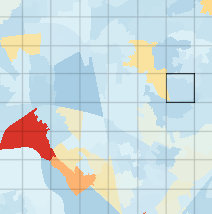
\includegraphics[width=0.3\linewidth]{images/highlightExample2}}~
\subfloat[Contour Highlight]
{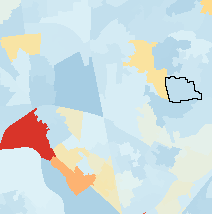
\includegraphics[width=0.3\linewidth]{images/highlightExample}}~
\subfloat[Cursor Concept]
{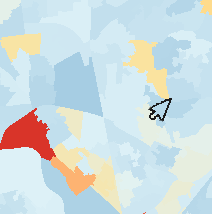
\includegraphics[width=0.3\linewidth]{images/highlightExample1}}
\caption{Three concepts for communicating requested area. The selected process was the contour highlight } \label{fig:highlight}
\end{figure}

\textbf{Communicating the target unit area to the user: } One of the most important factors of the experiment is to verify whether the user can accurately interpret the underlying color of an area of screen space. In order to do this, we need to accurately communicate the target area itself without obscuring or enhancing the area's color. This becomes non-trivial when perceiving an area of screen space at less than 1\%. We considered the use of a grid to quickly convey the target area. Although the grid could be effective with uniform size areas, the grid would become less accurate with non-uniform size areas. Grid granularity would also need to be taken into account and conditions in which cell labeling would become harder to communicate.
Using the mouse cursor to communicate the area to the user may allow the user to intuitively see the target area. The disadvantage of this is it could cause a wider variance in performance time, and the mouse pointer itself could cause occlusion. A super-imposed cursor could be added to the image to control mouse movement, however, this could still result in scenarios with multiple small areas close together being difficult to diagnose. Refer to Figure \ref{fig:highlight} for examples.

 We use Robinson's design criteria \cite{robinson2011highlighting} in order to select an identification criterion that does not alter or accentuate the value itself. We use style reduction highlighting using the lower alpha boundaries discussed in the area boundary design and give contour highlighting to outline the communicated area using a thicker black outline. We use a pixel thickness of 4 pixels to aid the use for smaller areas in order to reduce the effects of framing areas.
  On piloting the identification criteria, this alone was deemed to be insufficient causing users to overlook small areas. On top of these criteria, we added a blinking effect to help the user locate the target area, and render the highlighted color to something that stands out over the existing boundary. In this case, we use a black boundary which stands out from our color palette. The black outline blinks at 1Hz for a period of 1 second. In order to further aid the search for the highlighted area, we place a grey circle around the target area, where the target area sits in the center of the circle, and fills 10\% of the screen, and blinks with the black contour. See Figure \ref{fig:sample} (a). 


\textbf{Choice of Color Map: } 
Selecting the appropriate color map is an important decision when testing perception (refer to Section \ref{sec:related}). We use colorbrewer \cite{colorbrewer} due to its far-reaching application across geography and cartography, and acceptance with basic and advanced users \cite{brewer2003transition}. Colorbrewer is also created by geospatial visualization experts. We would like to ensure perceptual distances and therefore avoid the use of a sequential color map focused on a single hue. We can incorporate qualitative and diverging color maps for the color palette. Using Heer and Stone's color saliency test, we can see that qualitative color palettes tend to have better saliency, and therefore use this as a guideline \cite{heer2012color}. Although Tablaeu's color palette provides marginally better saliency, we use Colorbrewer's qualitative color map \cite{colorbrewer, tableau}. See Figure \ref{fig:color}.

\begin{figure}[t] \centering
\subfloat[]{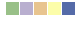
\includegraphics[scale=2]{images/clbrwr1}}~
\subfloat[]{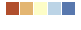
\includegraphics[scale=2]{images/clbrwr2}}~
\subfloat[]{
\includegraphics[scale=2]{images/tableau2}}
\caption{3 options for color mapping. (a) Colorbrewer's 5 color palette (qualitative). (b) Colorbrewer's 5 color palette (diverging). (c) Tableau 10 color palette (reduced to 5 for consistency). We use (a) for this study \cite{colorbrewer, tableau}.} \label{fig:color}
\end{figure} 


\textbf{Display Screen Resolution: }
Keeping resolution consistent is essential to experimenting with perception. Both digital resolution (display resolution) and physical resolution (monitor size) need to be consistent. In order to ensure this, we must forgo a mechanical turk testing environment and work in a controlled lab test environment. This is further explained in Section \ref{sec:equipment}.

\textbf{Lighting Conditions of Environment:}
We must consider the lighting as an important control variable when conducting this experiment. We make sure that the lighting environment stays the same by using a static study location, that uses interior lighting as the only lighting source. We also must consider the monitor's lighting settings, we do this by calibrating the screen using an International Color Consortium (ICC) profile. We provide a sample of presented question designs for T1 and T2 in Figure \ref{fig:sample}.

\begin{figure}[p]
\centering
\subfloat[T1 Sample]{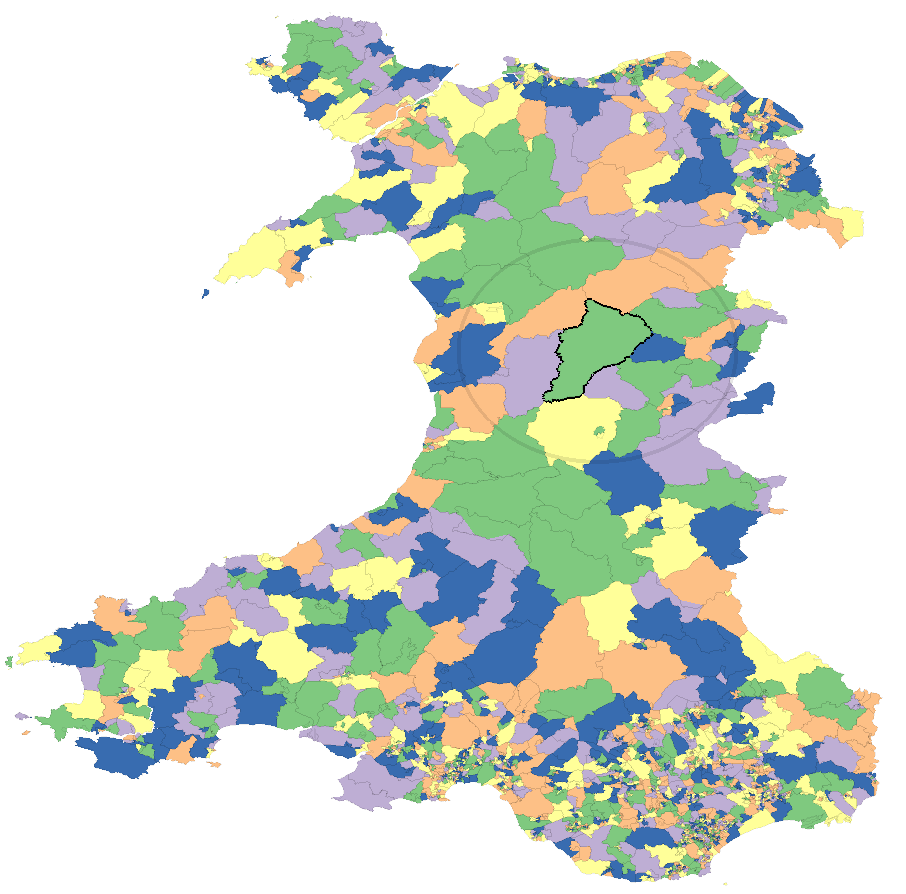
\includegraphics[width=0.6\linewidth]{images/sample}} \\
\subfloat[T2 Sample]{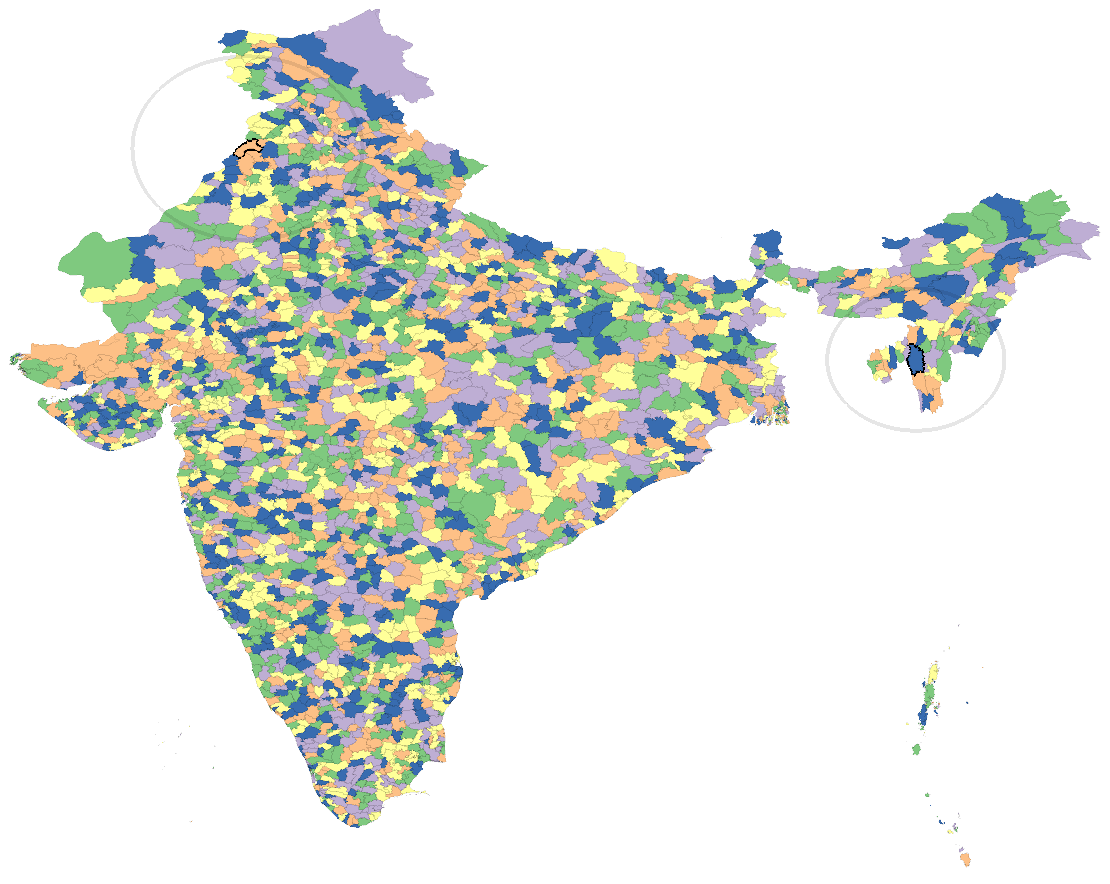
\includegraphics[width=0.8\linewidth]{images/samplet2}}
\caption{Sample questions for T1 and T2.} \label{fig:sample}
\end{figure}

\begin{figure*}[t]
\centering
\subfloat[Original]{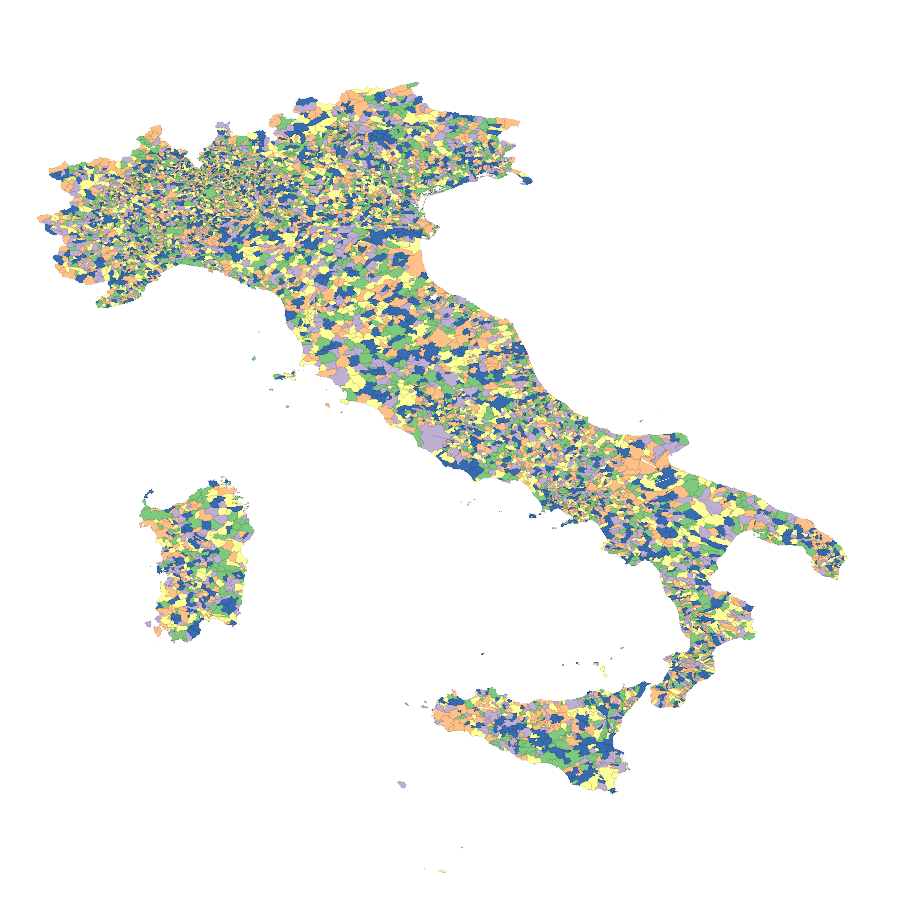
\includegraphics[width=0.3\linewidth]{images/0-000}} 
\subfloat[0.100\% Minimum Area Size]{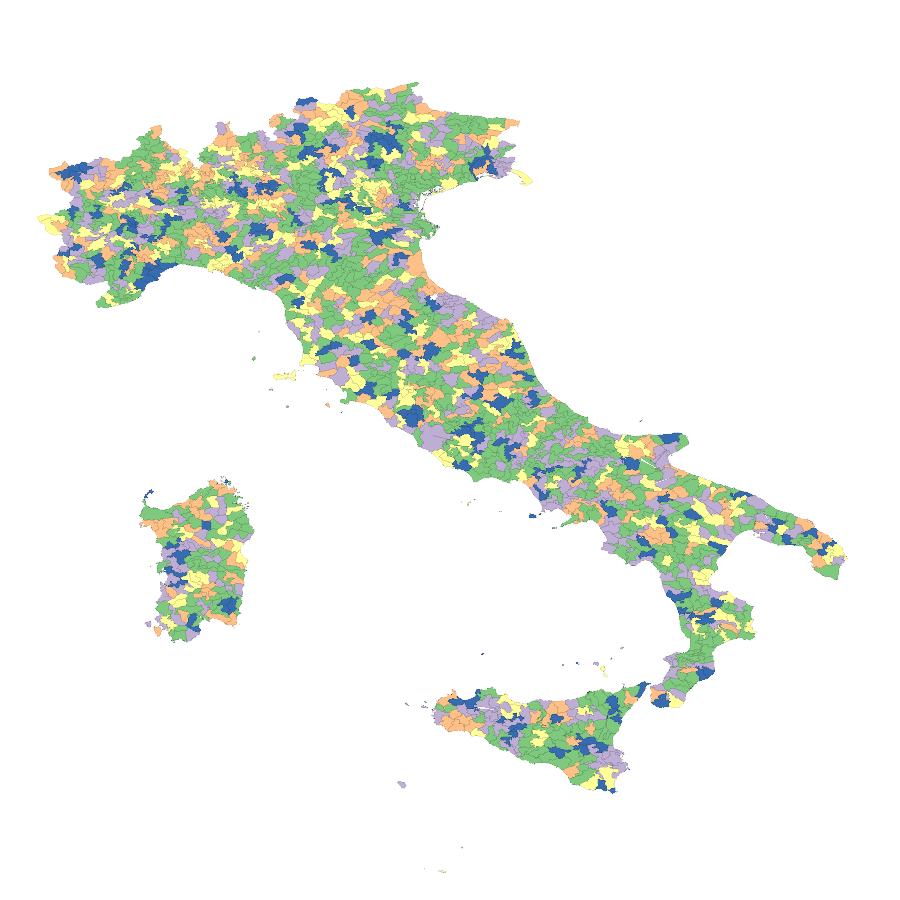
\includegraphics[width=0.3\linewidth]{images/0-100}} 
\subfloat[0.250\% Minimum Area Size]{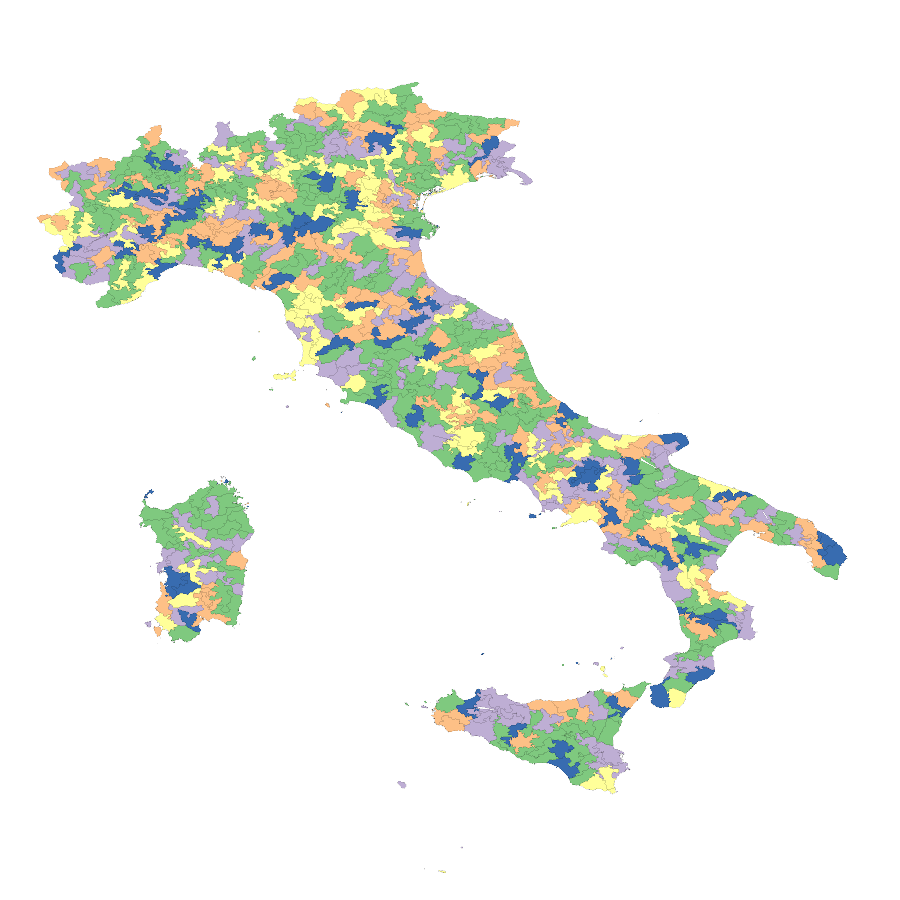
\includegraphics[width=0.3\linewidth]{images/0-250}}
\caption{Sample map designs using dynamic maps presented in Chapter \ref{chap:dcm} for T3.} \label{fig:samplet3}
\end{figure*}
\section{Perceivability Experiment} \label{sec:experiment}
In this section, we discuss the nature of the experiment including our designated equipment, experiment design, and stored experiment data.
\subsection{Equipment} \label{sec:equipment}
For this process, we use a standard Dell U2412M display resolution of 1920x1080p, on a screen size of 21". We then display the choropleth images to the subject as a static image 1200x960p. The desktop used to test this implementation features an Intel i5-4460 at 3.2GHz with 16GB of RAM and a GeForce GTX960. The test is run using the Qt Framework \cite{Qt}. For the ICC color profile, we use the Dell U2412M (Custom) color profile with suggested settings \cite{icc}.
\subsection{Procedure} \label{sec:process}
The experiment requires approximately 30 minutes per participant. We solicit ten participants who individually perform the tasks in this study. The subjects were gathered using an advertising campaign. The experiment is designed to test the perception of color conveyed by areas with a small screen space.  An instructive introduction explains what the test entails, what a choropleth is, how a task is completed, and sample questions. Some sample questions are used to test for the basic understanding of the tasks as well as a test for color blindness or eyesight problems. The sample questions provide a task where the largest area is used as the target. Test subjects who fail the training questions do not have their results used. For T1 a standard question presents a choropleth map image mapped by a color palette. There is one highlighted area in which the subject diagnoses the conveyed color. Each section of the color palette is presented as an option for the subject to select. The subject's color-choice answer is saved to a database for further analysis along with the true color of the area. These are saved as well as the performance time, choropleth identifier, area identifier, and the area's size in terms of pixels and screen space percentage. The experiment is run in task sets of 10, where each set provides a set of random choropleth maps and random unit area targets with a screen space ranging from 1 pixel upwards. When the set is complete we produce a short transitional state where we ask the participant for a confidence rating and ease of understanding rating. See Figure the Supplementary Material. Each task is associated with a random choropleth, random color from the color map, and randomized choice of a unit area on the choropleth in order to prevent learning effects. We run this for five sets.

T2 is presented indicating two unit areas on the same choropleth map. The user is asked to diagnose whether the units are the same color, or differ. After selecting their answer, the answer is saved as well as the same set of information in T1, for each area. This is run in sets of five, with ten tests per set. See Figure \ref{fig:sample} for sample images.

T3 is presented by showing a dynamic map presenting the same data using the Dynamic Choropleth Map procedure presented in Chapter \ref{chap:dcm}. We let the user dynamically select their preferred minimum screen space. The map for each position on the slider is split to enable options for the default map, moving up in increments of 0.001\% up to 0.01\%, and an increment of 0.01\% minimum screen space up to 0.25\%. The user will simply select the preferred size using the slider and a new map will replace it. This is done for five different comparisons, with the selected options being stored for further analysis. Refer to Figure \ref{fig:samplet3}. These maps will be given sequentially as we want to gather data for each of these maps, where the slider of each represents different constrained minimum areas.

\subsection{Stored Experimental Data} \label{sec:stored}
\begin{table}[b]
\centering
\rowcolors{2}{lightgray!10}{white}
\begin{tabularx}{0.78\linewidth}{|X|ccc|}
\hline 
\rowcolor{lightgray!30}
\textbf{Stored Data:} & \textbf{T1} & \textbf{T2} & \textbf{T3} \\ \hline
User ID & \cmark & \cmark & \cmark \\
Set ID & \cmark & \cmark & \xmark \\
Test ID & \cmark & \cmark & \xmark \\
Performance Time & \cmark & \cmark & \cmark \\
Map ID & \cmark & \cmark & \cmark \\
Target ID & \cmark & \cmark{\color{black} \textbf{x2}} & \cmark \\
Screen space for Target & \cmark & \cmark{\color{black} \textbf{x2}} & \xmark \\
Pixels for Target & \cmark & \cmark{\color{black} \textbf{x2}} & \xmark \\
User Selected Color & \cmark & \cmark & \xmark \\
Target Color & \cmark & \cmark & \xmark \\
Set Confidence & \cmark & \cmark & \xmark \\
Set Ease & \cmark & \cmark & \xmark \\
Slider Value & \xmark & \xmark & \cmark \\
\hline
\end{tabularx}
\caption{Table indicating the data saved for each task. Refer to Section \ref{sec:stored}. } \label{tbl:data}
\end{table}
Refer to Table \ref{tbl:data} for a visual breakdown of the stored experimental data. Data stored per task in T1 for analysis includes: map identifier, target area identifier, user-selected area color, target area color, task time, task identifier, and set identifier.
T2 saves all of the T1's information, but with the additional data for the second target area. For both T1 and T2, we store the set identifier, confidence level, and difficulty level per set.
For T3 we store: task identifier, task time, and preferred screen space identifier.
T1 does not store any information for target two as the task only focuses on one target area. T2 includes the most data saved. T3 does not save any information for sets, screen space of targets (as targets already refer to screen space), pixels, or the target answer, as this is used to test preference. Therefore we save the value selected using an interactive slider. See Table \ref{tbl:data}.

\section{User-Study Results} \label{sec:results}
In this section, we discuss the results of three tasks which include diagnosing the color value of areas on a choropleth map, comparing the color of areas on a choropleth map, and determining user preference for choropleth maps concerning minimum area size. The task included 10 participants with 50 data samples per participant for both T1 and T2, and 5 data samples per participant for T3 (from a selection of 130 potential candidates). Of the participants, we use an unconstrained sample of users from both genders, a range of ages (18-35), at different expertise levels. Candidates were provided with {\textsterling}10 amazon vouchers after the completion of the study's completion. None of the participants failed the screening process. 
\subsection{T1 Analysis}
\begin{figure}[p]
\centering
\subfloat[]{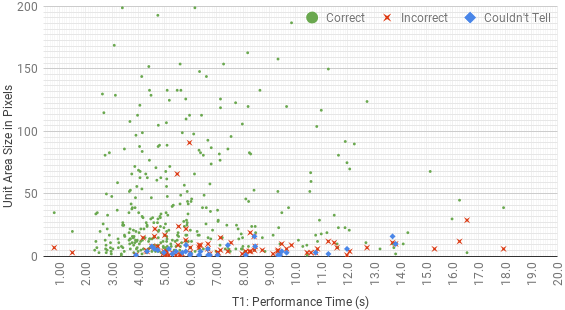
\includegraphics[width=1\linewidth]{images/T1Scatter}} \\ \vspace{-0.35cm}
\subfloat[]{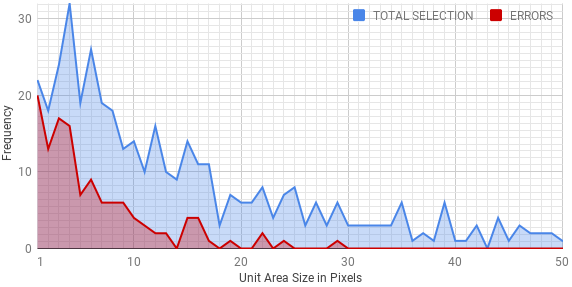
\includegraphics[width=1\linewidth]{images/T1Accuracy}}
\caption{\textbf{T1:} (a) A scatter plot depicting the correlation between performance time (seconds) and area size (in pixels). Color is mapped to Answer Category (green for the correct answer, red for an incorrect answer, blue for `couldn't tell'). (b) Area chart presenting the T1 error rate based on area size measured in pixels, where the blue area represents the total samples per area size, and the red area represents the error per sample.} \label{fig:t1results}
\end{figure}
Task 1 involved the user determining the color of highlighted areas. Each user completed the task with 50 data samples, excluding outliers for a total of 500 data samples across all users. Of these 500, we use 465 of these for analysis, filtering out areas that are over 200 pixels in size, or outliers in terms of performance time (see Chapter \ref{chap:conclusion}). For T1 we present our findings using a scatter plot and area chart (Figure \ref{fig:t1results}). The unit plot displays the relationship between performance time, unit area size, and user results. We can see a large distribution of results where the user correctly interpreted the color mapped to the area. For incorrect results, we see that the results primarily fall very close to 0. On top of this, we identify when a user selects the `couldn't tell' option. This seems to fall along the lower half of the incorrect distribution. In terms of performance time, there is a clear gap between 0-2 seconds. This seems to be related to user search time, and the highlight animation. This is followed by another 2 seconds where there is a noticeable gap in incorrect answers. This might be influenced by pre-attentive processing. The area chart presents the accuracy of T1 error based on a unit area. We also provide a histogram to present the frequency of size representation in the study. For T1, we see clearly that accuracy is particularly low below 5 pixels in size. With a range of error just over 90\% for 1 pixel. We see from this chart that the error becomes prevalent under 10 pixels. \\
\textbf{Statistical Analysis: } We use our results of T1 in our analysis of H1 (size vs error) and H2 (size vs time) using the Pearson correlation co-efficient where $\alpha$ = 0.05. As our sample size favors smaller pixels due to the random nature, we use a normalized error rate to calculate the relationship between area size and error.  We conclude using Pearson's correlation co-efficient that there is a relationship between area size and error rate, where r(50) = -0.77%04910537
. This supports our hypothesis H1. For H2, we conclude there is a relationship between area size and performance time, where r(466) = -0.325%3428361
. This supports our hypothesis H2. Due to this, we can verify that our first two hypotheses are supported statistically by our results for T1. 

\subsection{T2 Analysis}
Task 2 involves comparing 2 highlighted areas in order to diagnose whether they are mapped to the same color value. Each user completed the task with 50 data samples for a total of 500 data samples across all users. Of these 500 we use 490 of these for analysis, filtering out areas that are over 200 pixels in size, or outliers in terms of performance time (see Chapter \ref{chap:conclusion}).  We produce similar graphs to facilitate comparison between T1 and T2 (see Figure \ref{fig:t2results}). Similarly to T1, correct answers exhibit a wide distribution of pixels and performance time, however, we find that users were far more liberal with the use of of the 'cannot tell' option. This suggests that the binary comparison was more difficult than the selection of colors, confirming the assumption that color salience may have been an important factor to consider.

\begin{figure}[p]
\centering
\subfloat[]{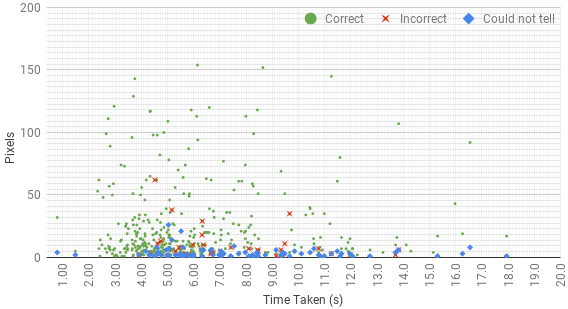
\includegraphics[width=1\linewidth]{images/T2Scatter}} \\ \vspace{-0.35cm}
\subfloat[]{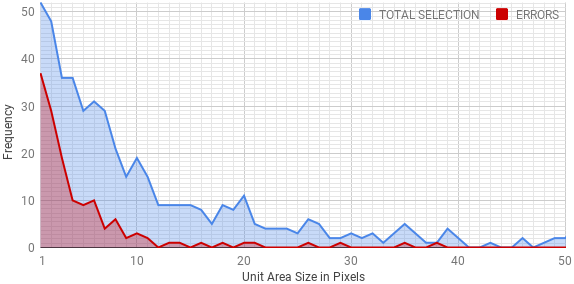
\includegraphics[width=1\linewidth]{images/T2Accuracy}}
\caption{\textbf{T2:} (a) Scatter Plot depicting the correlation between performance time (seconds) and area size (pixels) of the smallest target area. Color is mapped to user performance (green for correct answer, red for incorrect answer, blue for could not tell). (b) Area chart presenting the T2 error rate based on area size measured in pixels, where the blue area represents the total samples per area size, and the red area represents the error per sample.} \label{fig:t2results} \vspace{-0.6cm}
\end{figure}

In terms of accuracy, we can see that the error rate for T2 was less extreme for small area sizes, but has a slightly higher distribution which leads to error up to 39 pixels (although 38 pixels has only one test case, 35 pixels has a better sample size). The lower error rate at smaller sizes could be related to a couple of visual features. First, as there are 5 map-able colors, when diagnosing colors in T2, a decision can be made by testing the contrary. A user may not be able to distinguish color in T1, however, if they can distinguish that the two colors are not the same without distinguishing the correct color, they can effectively answer the question. We must also consider that although we provide and encourage the use of the `couldn't tell' button, some users compared this to a test and therefore ignored the button. For T1, guessing a correct answer has a 1/5 chance of being correct, however, selecting the `no' option has a 4/5 chance of being a correct answer in T2.\\
\textbf{Statistical Analysis: } We use our results of T2 in our analysis of H1 (size vs error) and H2 (size vs time) using the Pearson correlation co-efficient where $\alpha$ = 0.05, similarly to our analysis of T1. We follow the same convention to analyze error as in T1, by using normalized error. From this analysis, we conclude using Pearson's correlation co-efficient that there is a relationship between area size and error rate, where r(50) = -0.433%5144942
. This supports our hypothesis for H1. For H2, we conclude there is a relationship between area size and performance time, where r(490) = -0.358%1890952
. This also supports our hypothesis H2. As T1 and T2 both support the hypotheses of H1 and H2, we can be confident that our hypotheses for each are evident.
\subsection{T3 Analysis}
For T3, we allow the user to select the most "useful" map from a set of fixed-locale choropleths which constrain areas size, using the Dynamic Choropleth Map procedure presented in Chapter \ref{chap:dcm}. We defined "useful" as being `your preference of area size against the data relayed, where larger areas provide more uncertain data'. A histogram is used to visualize the frequency of selection for T3 and the results of this task are quite unexpected (see Figure \ref{fig:t3results}).  We expected that the preference would be found at the lower end of the spectrum, however, over half of the study participants selected the largest possible enforced minimum screen space. On top of this, our pilot study prompted us to increase the number of selectable areas closer to the default screen space which did not reflect any results in the study. This may have been caused by the discrepancy in size variation between the first 10 selections, and the following selections. In order to rectify this, a follow-up study may be necessary that shows screen space on a logarithmic scale to remove that type of bias, or a larger selection of choices, that is quantized into bins. Unlike H1 and H2, we cannot effectively run statistical analysis on our finding due to the subjective nature of the task. However, our observations do show evidence to support hypothesis H3. A more thorough investigation of this task is a good area for future work.
\begin{figure}[t]
\centering
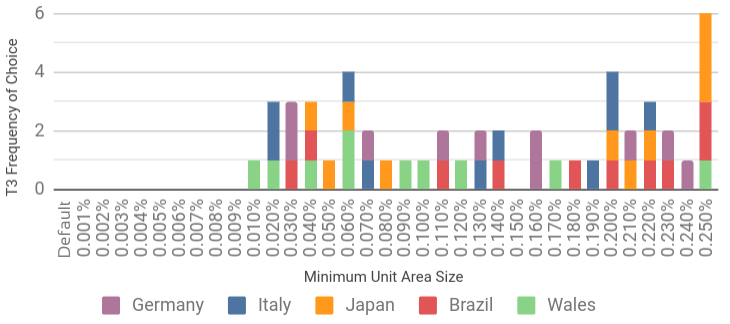
\includegraphics[width=1\linewidth]{images/T3}
\caption{\textbf{T3:} Histogram presenting the frequency of minimum unit area size preference, where the preference is defined as `your preference of area size against the data relayed, where larger areas provide more uncertain data'.} \label{fig:t3results} \vspace{-0.8cm}
\end{figure}

\subsection{Anecdotal Results}
During the period of testing, there were a few interesting observations we noticed. We found that users were generally caught off guard by the difficulty of the test, although the random selection of areas was mentioned, some users believed that this was not the case, leading to the conclusion that many are unaware of the frequency of small areas. To continue with this, users tended to feel like they had performed poorly, making statements remarking the difficulty. Some users regarded surprise at the difficulty of T2, suggesting that they believed it would be easier to identify whether two colors would be the same, but found themselves in situations where it was difficult to identify either color. For T3, one user explained that his decision for larger areas was based on the fact that they prefer islands to consist of only one area, which suggests the users' preferred minimum screen space could be related to area contiguity.

%\section{Supplementary Material}
%We include supplementary material that provides high-resolution images of the scatter plots included. We also provide a video (\url{https://bit.ly/2M9wIvY}) previewing a demonstration of the user-study in action.

%\section{Limitations \& Future Work} \label{sec:limitations} \label{sec:limit}
%There are some limitations to the study we review. The first we must consider is some error in performance time. Although we record performance time as a variable, we concluded that users would not be tasked to complete questions under a time limit. This was due to the assumption that this may cause unnecessary strain on the user which would lead to higher error. Thus there is a larger distribution in task time than anticipated caused by human factors including participants: re-adjusting posture, asking questions, or making comments. We found boundary design to be a bigger factor for small sizes than anticipated. In the pilot study, we found that users had a much better accuracy overall, and comments were made about the area's color changing. This was actually due to the boundary's framing of the pixel, enhancing the perception of color based on the surrounding black contour. We try to control this as closely as possible, however, this could be examined further in a follow-up study. Finally, as we use real-world maps and areas, we do not control the aspect ratio of the areas, which may lead to more error in some situations such as narrow areas. This is an aspect that can be explored in an alternative study. Future work also includes a more in-depth statistical analysis of T1 and T2.

\section{Conclusion} \label{sec:conclusion}
We conduct a preliminary study to evaluate perceptual evaluation of performance error, performance time, and preference of area's relative to size in choropleth maps. We hypothesize that the smaller the size of a unit area, the higher the error rate of perceiving the correct underlying color category; the smaller the unit area, the more time required to perceive its color; and the user will prefer choropleth maps with a larger minimum size over those with smaller sizes. Particularly, users will prefer a trade-off between area resolution in favor of legibility. For these three statements, we support the first two using Pearson's r to show a relationship between the variables, with strong observations for the third that give an initial understanding of how users' perceive the relationship between area size and data on a choropleth map. We give a recommendation of at least 10 pixels displayed for each area to be accurately interpreted. This translates to a percentage of $4.82253x10^{-4}$ for estimation on similar screens.

%\section{Acknowledgements}
%We would like to thank KESS for contributing funding towards this endeavor. Knowledge Economy Skills Scholarships (KESS) is a pan-Wales higher level skills initiative led by Bangor University on behalf of the HE sector in Wales. It is partially funded by the Welsh Government's European Social Fund (ESF) convergence programme for West Wales and the Valleys. We also thank GoFore UK for contributing funds to this endeavor. We thank Dylan Rees, Richard Roberts, and Jamie Gilbertson for proofreading this paper.

\begin{figure}[t]
 \centering
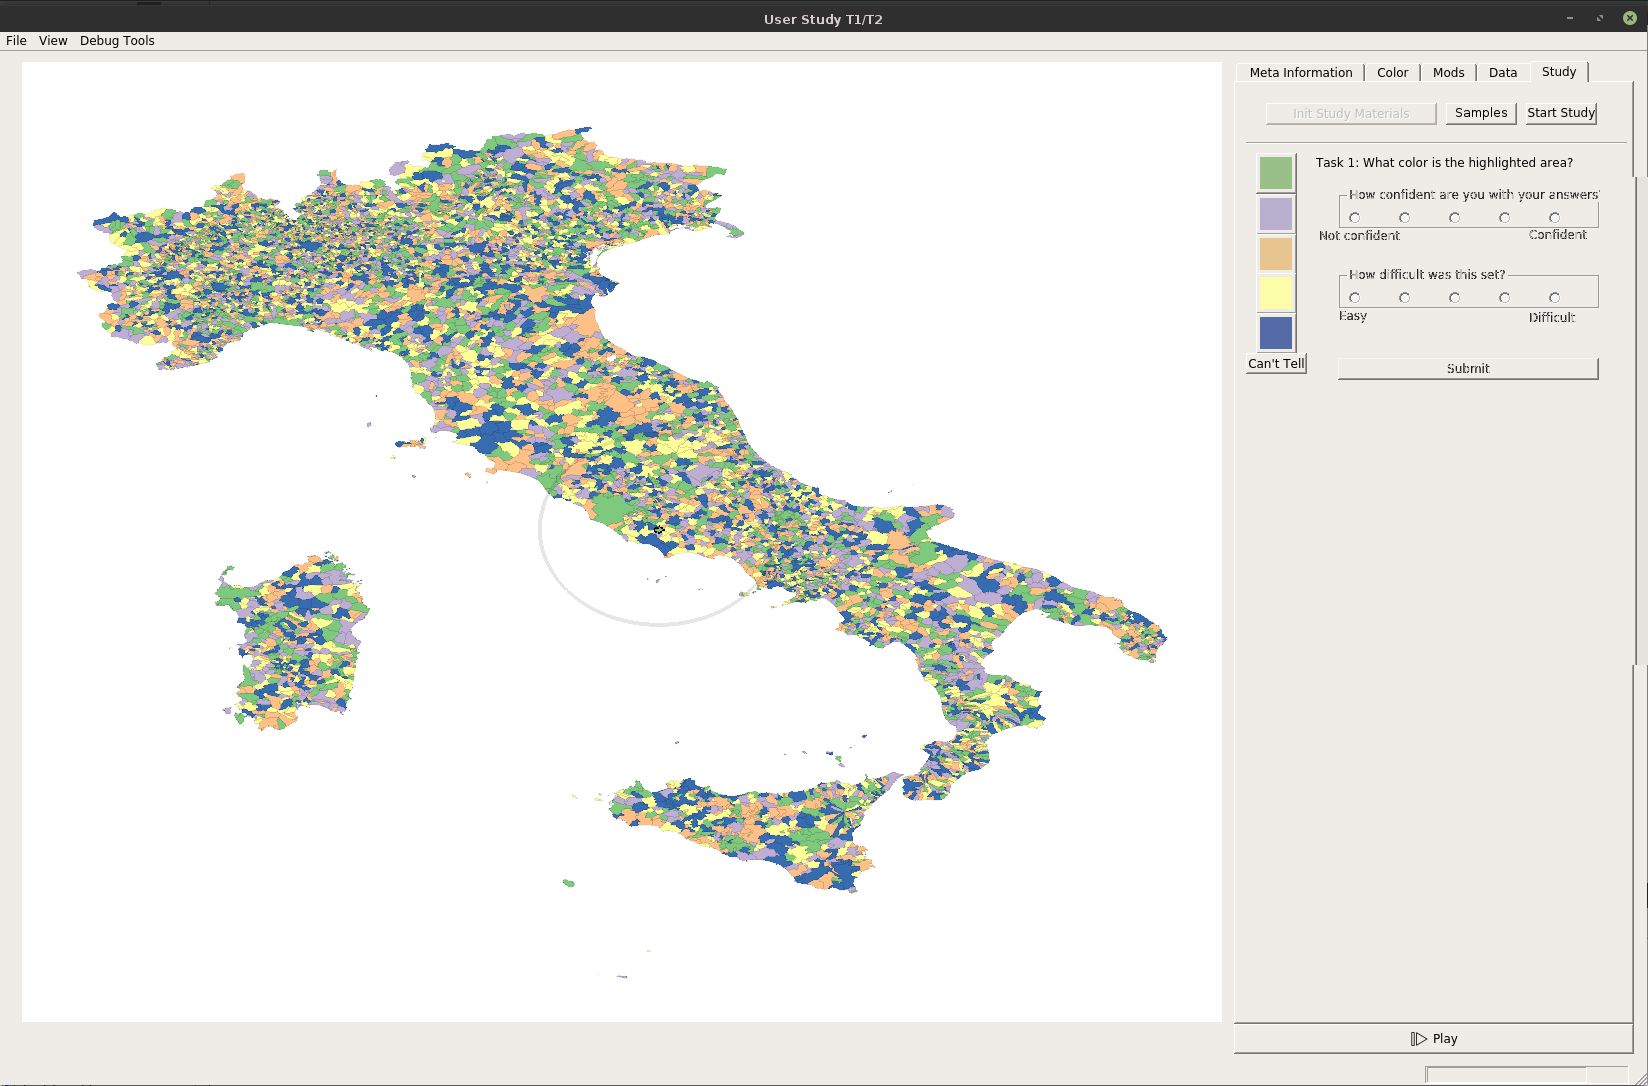
\includegraphics[scale=0.35, angle=90]{images/T1.png}
\caption{Sample question for T1 presenting in application, including user interface. This sample shows a more realistic question than the samples shown in the Main text (selected to present clearer examples).} \label{fig:t1}
\end{figure}
\begin{figure}[t]
 \centering
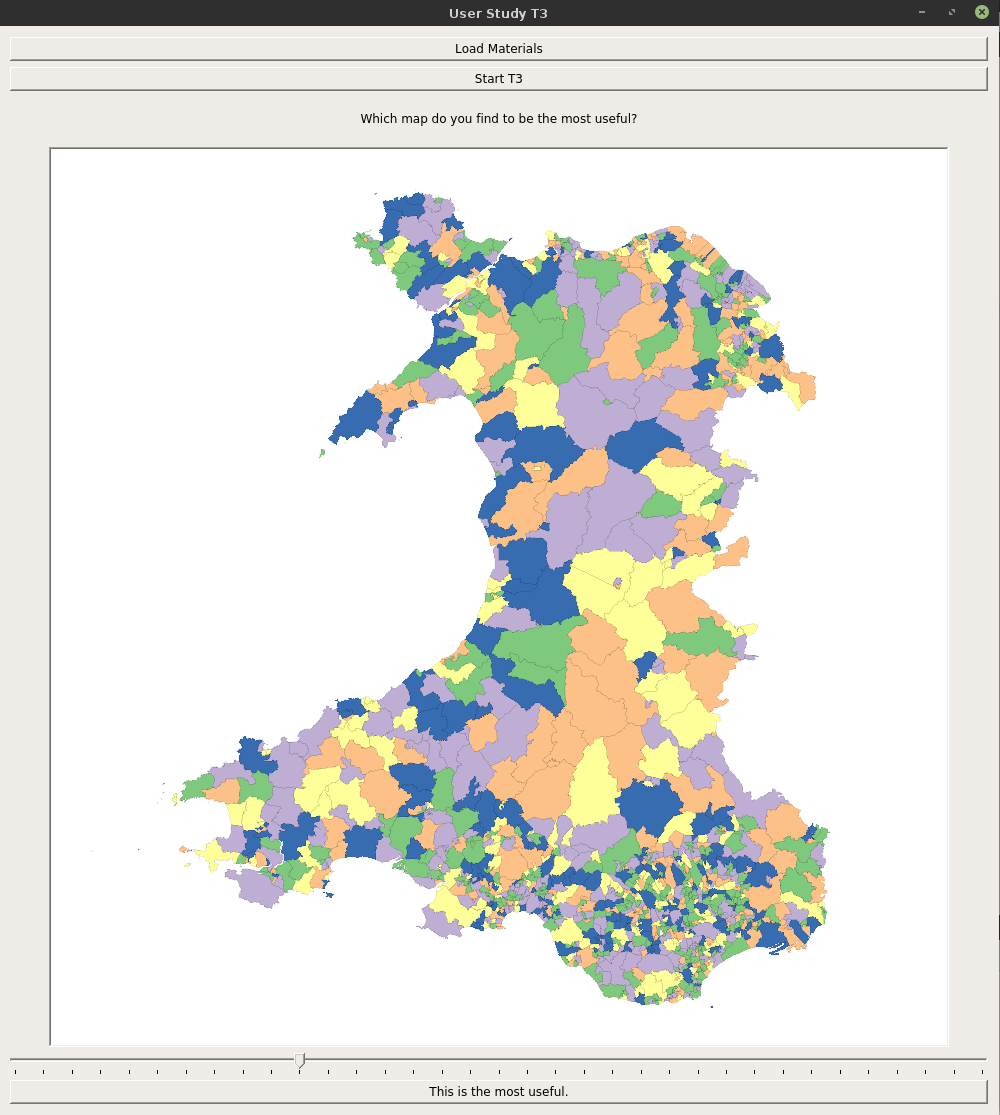
\includegraphics[width=1\textwidth]{images/T2.png}
\caption{Sample question for T3 presenting in application, including user interface.} \label{fig:t3}
\end{figure}

